\documentclass[onecolumn, draftclsnofoot,10pt, compsoc]{IEEEtran}

\usepackage{graphicx}
\usepackage{url}
\usepackage{setspace}
\usepackage{geometry}
\usepackage{listings}
\usepackage{color}
\usepackage{etoolbox}
\usepackage{pdflscape}
\usepackage{titling}

\geometry{textheight=9.5in, textwidth=7in}

\def\name{Group 26}


\title{Homework 4 Report\\\large CS444 Fall17}
\author{Zach Lerew, Rohan Barve\\\large Group 26}
\date{\today}

% Syntax highlighting
\lstset{
  basicstyle=\footnotesize,        % size of fonts used for the code
  breaklines=true,                 % automatic line breaking only at whitespace
	frame = single,                  % code framing
}



\begin{document}
  % Title page
  \maketitle

	\begin{titlingpage}
		\begin{abstract}
			\noindent Homework 4 involved modifying the existing slob allocator for the linux yocto kernel to use a best fit algorithm in order to compare fragmentation rates between a first -fit algorithm in slob which is the default against a best -fit.  We also had to learn how to write system calls and how to test a slob allocator. In computer storage, fragmentation is a phenomenon in which storage space is used inefficiently, reducing capacity or performance and often both. The exact consequences of fragmentation depend on the specific system of storage allocation in use and the particular form of fragmentation. In many cases, fragmentation leads to storage space being "wasted", and in that case the term also refers to the wasted space itself.

		\end{abstract}
	\end{titlingpage}

  \pagenumbering{arabic}
  \clearpage
  \singlespace

	% Document body
	\section*{Design}
  For this assignment, the team went online to research what a best fit algorithm is and how it can be implemented. Upon conducting research the team decided to implement this version of the best fit algorithm:
		Algorithm for allocate (n)
		size(block) = n + size(header)
		Scan free list for smallest block with nWords >= size(block)
		If block not found
   				 Failure (time for garbage collection!)
		Else if free block nWords >= size(block) + threshold*
    				Split into a free block and an in-use block
    				Free block nWords = Free block nWords - size(block)
    				In-use block nWords = size(block)
    		Return pointer to in-use block
	Else
    		Unlink block from free list
    		Return pointer to block

*Threshold must be at least size(header) + 1 to leave room for header and link
Threshold can be set higher to combat fragmentation
Allocation time is O(K) (K = number of blocks in free list)

This algorithm was found on Rochester Institute of Technology's CS website concerning heap and garbage collection.


	\section*{Questions}
	\subsection*{1.What do you think the main point of this assignment is?}
	The main point of this assignment was to learn how to write system calls and continue to develop
	 kernel coding skills. The purpose was to give us an idea of how different storage algorithms can affect the level of fragmentation suffered when allocating memory from the slob allocator.

	\subsection*{2.How did you personally approach the problem? Design decisions, algorithm, etc.}
	The way our team approached this problem was first configure our current kernel to first use the slob allocator as the default is slab. Then we modified the slob.c file to include 2 system calls and fixed many compiler errors. Next we rebuilt the kernel and wrote a kernel module to test the slob allocator by having our module call kmalloc and kree. The kmalloc interface is built on top of the slob allocator and this is the best way to test it by calling kmalloc and kfree in a loop. Next we wrote a simple program that gives us the fragmentation rates for the default first -fit algorithm that exists in slobc.
		Once that was done, we tried to implement the best fit algorithm as closely as possible to the design we found which has been outlined above.

	\subsection*{3.How did you ensure your solution was correct? Testing details, for instance.}

	\begin{enumerate}

	\item Source environment
	\begin{lstlisting}
source <environment-file>
\end{lstlisting}

	\item Clean and build kernel
	\begin{lstlisting}
cd linux-yocto-3.19
make clean && make -j4 all
\end{lstlisting}

  \item Run qemu using this command, which enables networking and file transfer with Description
	\begin{lstlisting}
qemu-system-i386 -redir tcp:<PORT>::22 -nographic -kernel linux-yocto-3.19/arch/x86/boot/bzImage -drive file=core-image-lsb-sdk-qemux86.ext4 -enable-kvm -usb -localtime --no-reboot --append ``root=/dev/hda rwconsole=ttyS0 debug``
\end{lstlisting}

\item In another terminal, Build module
\begin{lstlisting}
cd linux-yocto-3.19/kernel4/
make
\end{lstlisting}

	\item In another terminal, transfer module to VM with SCP
	\begin{lstlisting}
cd linux-yocto-3.19/kernel4
scp -P <PORT> mod.ko root@localhost:~
scp -P <PORT> test.c root@localhost:~
\end{lstlisting}

	\item Insert module
	\begin{lstlisting}
cd ~
insmod mod.ko
lsmod
\end{lstlisting}

  \item Compile testing script in QEMU
  \begin{lstlisting}
cd ~
gcc test.c
\end{lstlisting}

  	\item Test module to confirm that it works, you should see messages regarding free space, total space, and fragmentation involved. Compare to images below.
  	\begin{lstlisting}
./a.out
\end{lstlisting}

  \item Remove module
  \begin{lstlisting}
rmmod mod.ko
\end{lstlisting}


Best Fit:

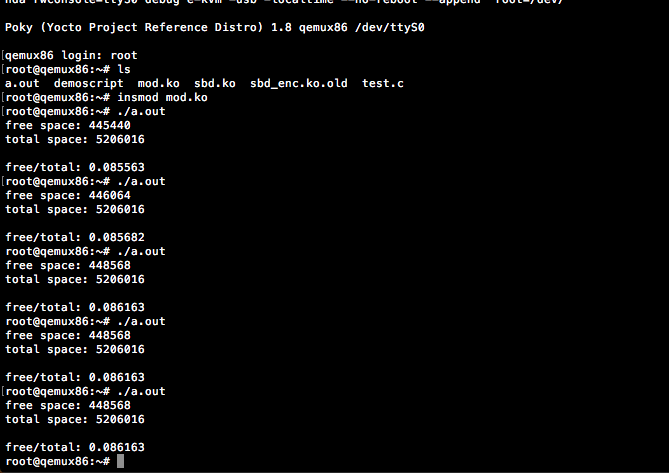
\includegraphics[width=\linewidth]{best-fit.png}

First Fit:

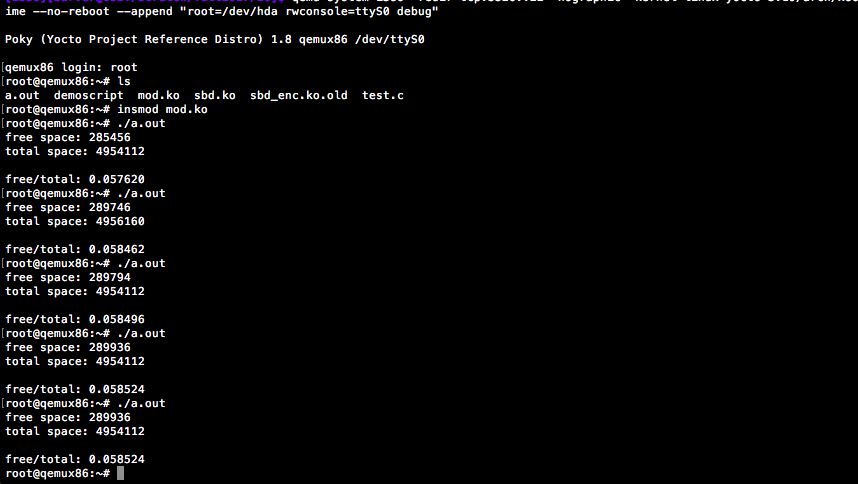
\includegraphics[width=\linewidth]{first-fit.png}


	\end{enumerate}

	\subsection*{4.What did you learn?}
  In this assignment we learnt how to write system calls, understand the slob allocator interface and how memory is allocated for general purpose operations. We also got practise in modifying an existing kernel file and learnt how frustrating this process can be. It took us many hours of research to try to implement a best-fit algorithm for the slob allocator  we had to work off of.


  \section*{Work log}
    \begin{center}
      \begin{tabular}{ |c|c|c| }
        \hline
        Date & Author & Commit Description \\
        \hline
        2017-12-1 & Zach Lerew & Merged writeup content and tar.bz2 zipped project \\
        2017-12-1 & Zach Lerew & Added linux patch and server only files \\
        2017-12-1 & Rohan Barve & Added test program to compare fragmentation rates \\
        2017-12-1 & Rohan Barve & Added slob kernel testing module \\
        2017-12-1 & Rohan Barve & Fixed compiler errors for slob.c to get it to work with yocto version 3.19 \\
        2017-11-30 & Rohan Barve & Added working copy of slob.c with best fit algo \\
        2017-11-29 & Zach Lerew & Added design details to writeup \\
        2017-11-28 & Zach Lerew & Added hw4 writeup copied from hw3 \\
        \hline
      \end{tabular}
    \end{center}


  %References
  \bibliography{ref}
  \bibliographystyle{IEEEtran}

\end{document}
